\chapter{Proposed algorithm}
\label{cha:proposed_algorithm} % (fold)
Our aim is to learn from multiple source tasks using shared knowledge in order to have a better performance on a target task than when we wouldn't train on source tasks.
While a version of the algorithm was implemented where the source tasks are executed sequentially for each episode, the focus is on a version where source tasks are learned simultaneously.
More specifically, we combine the A3C algorithm \parencite{Mnih2016AsynchronousLearning} with the transfer learning algorithm in \cite{Isele2016UsingLearning}.
This is done by executing A3C using tasks defined by different environment parameters instead of exactly the same ones and training them using both shared knowledge and knowledge that is specific to the task.\\

Our approach only uses a latent basis over the policy space instead of using one over the policy space and another one over the descriptor space like in \cite{Isele2016UsingLearning}.\\
Each task uses 2 sets of parameters in its artificial neural network: the shared knowledge base and the sparse coefficients (also called \emph{sparse representation}). As the name suggests, the shared knowledge base is used by every task and can capture knowledge that is common amongst those tasks. Each task has its own sparse coefficients over this shared basis. Using these sparse coefficients, each task can represent differences from the common knowledge in order to better perform on its environment.\\
For a task $t$, we can reconstruct the policy using the shared basis $L$ and the sparse coefficients over this basis for that specific task $s^{(t)}$: $\theta^{(t)} = Ls^{(t)}$, with $\theta^{(t)} \in \mathbb{R}^d$, $L \in \mathbb{R}^{d \times k}$ and $s^{(t)} \in \mathbb{R}^k$. The policy can then be combined with the state or features extracted from it by taking the weighted sum and passing it through a non-linearity, in this case the softmax function described in Section~\ref{sub:softmax}.
This results in a probability for each action.\\
The architecture of the network used for one task is visualized in Figure~\ref{fig:algonn}.
\begin{figure}[htb]
    \centering
    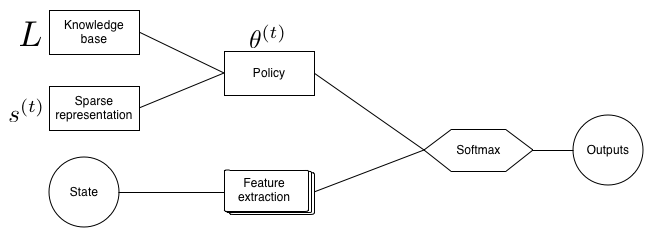
\includegraphics[width=.9\linewidth]{images/knowledge_transfer.png}
    \caption[Artificial neural network architecture used in our approach]{Artificial neural network architecture used in our approach. The sparse representation $\theta^{(t)}$ is different for every task $t$, while the same knowledge base is used for every task.}
    \label{fig:algonn}
\end{figure}\\

The source tasks can be learned in two ways, either sequentially or in parallel.
In the sequential way, we collect trajectories and calculate the gradients for every task after another.
These gradients include both those for the sparse representation and for the knowledge base.
They are calculated for every episode of a task like in the \textit{REINFORCE} algorithm (explained in Section~\ref{sub:rl:policy_gradient}), i.e.\ with likelihood ratios using discounted rewards as a sample for the $Q$ values of the policy.
After evaluating every task, we sum and apply all of their gradients.
The learning process for the source tasks stops when a certain number of updates have been applied.\\
In the parallel way, all source tasks are learned at the same time, each executing a certain number of updates.
Trajectories are collected for each task continuously and its gradients are applied immediately after they are calculated.
This means that they are not first summed up like in the sequential method.\\
The resulting pseudo code for the source tasks learned using the parallel method can be seen in Algorithm~\ref{algo:ownsource}.\\
\begin{algorithm}[H]
\DontPrintSemicolon
\emph{// Assume global knowledge base $L$ and global shared counter $H \gets 0$}\;
Initialize thread-specific parameter vector $\theta^{(t)}$\;
Initialize thread step counter $h\gets 1$\;
\Repeat{$H > H_{max}$}{
    $\theta^{(t)} \gets Ls^{(t)}$\;
    Reset gradients: $d\theta^{(t)} \gets 0$\;
    $h_{start} \gets h$\;
    Initialize state $x_h$\;
    \Repeat{terminal $x_h$ \textbf{or} $h-h_{start} = h_{max}$}{
        Perform $a_h$ according to policy $\pi(a_h\vert x_h;\theta^{(t)})$\;
        Receive reward $r_h$ and new state $x_{h+1}$\;
        $h \gets h + 1$\;
        }
    \For {$i \in \{h-1,\dots,h_{start} \}$} {
        Accumulate gradients w.r.t. $L$: $dL \gets dL+ \alpha \nabla_{L} \log \pi_{\theta^{(t)}}(x_i,a_i)v_i$\;
        Accumulate gradients w.r.t. $s^{(t)}$: $ds^{(t)} \gets ds ^{(t)}+ \alpha \nabla_{s^{(t)}} \log \pi_{\theta^{(t)}}(s_i,a_i)v_i + L_1(s^{(t)})$\;
    }
    Perform asynchronous update of $L$ using $dL$\;
    Perform update of $s ^{(t)}$ using $ds ^{(t)}$\;
    $H \gets H + 1$\;
}
\caption[Asynchronous knowledge transfer agent for a source task]{Asynchronous knowledge transfer agent for a source task.}
\label{algo:ownsource}
\end{algorithm}

After learning the source tasks, the knowledge base that they jointly learned is transferred to the target task.
This task then separately learns and executes updates for a number of episodes.
The pseudo-code for the target task is shown in Algorithm~\ref{algo:owntarget}.\\
\begin{algorithm}[htb]
\DontPrintSemicolon
\emph{// Assume global knowledge base $L$}\;
Initialize task-specific sparse representation $s^{(t)}$\;
Initialize thread step counter $h\gets 1$\;
$H \gets 0$\;
\Repeat{$H > H_{max}$}{
    $h_{start} \gets h$\;
    Initialize state $x_h$\;
    \Repeat{terminal $x_h$ \textbf{or} $h-h_{start} = h_{max}$}{
        Perform $a_h$ according to policy $\pi(a_h \vert x_h; L  s^{(t)})$\;
        Receive reward $r_h$ and new state $x_{h+1}$\;
        $h \gets h + 1$\;
        }
    \For {$i \in \{h-1,\dots,h_{start} \}$} {
        Accumulate gradients w.r.t. $s^{(t)}$: $ds^{(t)} \gets ds^{(t)} + \alpha \nabla_{s^{(t)}} \log \pi_{s^{(t)}}(x_i,a_i)v_i + L_1(s^{(t)})$\;
    }
    Perform update of $s^{(t)}$ using $ds^{(t)}$\;
    $H \gets H + 1$\;
}
\caption[Knowledge transfer agent for the target task]{Knowledge transfer agent for the target task.}
\label{algo:owntarget}
\end{algorithm}
% section proposed_algorithm (end)
